\documentclass{article}
\usepackage[english]{babel}
\usepackage[utf8]{inputenc}
\usepackage{amsmath}
\usepackage{interval}
\usepackage{array}
\usepackage[table]{xcolor}
\usepackage{graphicx}
%--\renewcommand{\arraystretch}{2.5}
%--\arrayrulecolor[HTML]{DB5800}
%--\usepackage{float}
%--\usepackage{longtable}
%--\usepackage{rotating}
%--\usepackage{booktabs}
%--\usepackage{caption}

\usepackage{listings}

\usepackage{hyperref}
\hypersetup{
	colorlinks,
	citecolor=black,
	filecolor=black,
	linkcolor=black,
	urlcolor=black
}
\DeclareUnicodeCharacter{2212}{-}
\begin{document}


\begin{titlepage}
      \centering
      \begin{figure}
            \begin{center}
                  
\includegraphics[width=0.6\textwidth]{images/logo_polimi.png}
            \end{center}
      \end{figure}
      \vfill
      {\scshape\LARGE Numerical Analysis for Machine Learning\\Academic Year 2021 - 2022 \par}
      
      
      \vfill
      \newcommand{\HRule}{\rule{\linewidth}{0.3mm}}
      \centering
      \HRule \\[0.4cm]
      \huge  movieRecommendation\\% Title of your document
      \HRule \\
      \vspace{1cm}
      {\Large Sofia \textsc{Martellozzo} \quad Matteo \textsc{Nunziante} \par}
      \vfill
      {\large Professor\par
          Edie \textsc{Miglio}}
\end{titlepage}


\newpage
\renewcommand\contentsname{Contents}
\tableofcontents

\newpage

%------------------------------------------%
\section{Introduction}

With the advent of the internet today, we are witnessing an enormous information overload. This exponential growth in data results in difficulty organizing and analyzing this basic information but opens up new avenues on the paths of knowledge. The question is no longer to have the information but to find the relevant information simultaneously; from there, recommendation systems were born.\\ 
\textbf{Recommender System} is a system that seeks to predict or filter preferences according to the user’s choices. Recommender systems are utilized in a variety of areas including movies, music, news, books, research articles, search queries, social tags, and products in general. 
Recommender systems produce a list of recommendations in any of the two ways :
\begin{itemize}
      \item \textbf{Collaborative filtering}: Collaborative filtering approaches build a model from the user’s past behavior as well as similar decisions made by other users. This model is then used to predict ratings for items that users may have an interest in.\\
      \begin{figure}[h]
            \begin{center}
                  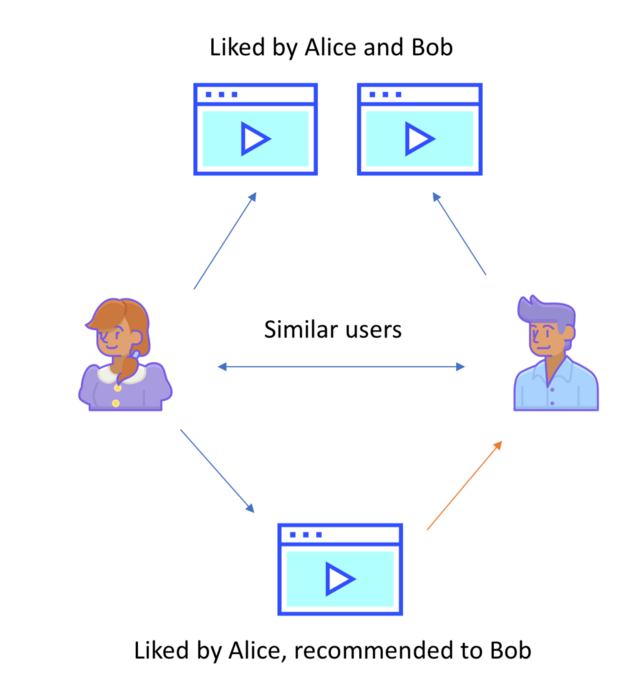
\includegraphics[width=0.5\textwidth]{images/Collaborative filtering.png}
            \end{center}
      \end{figure}\\
      The \underline{advantages} of this approach are:
      \begin{itemize}
            \item Domain knowledge not required: The system does not required a domain knowledge because is based only on item ratings.
            \item Serendipity: The model can help users discover new interests. In isolation, the ML system may not know the user is interested in a given item, but the model might still recommend it because similar users are interested in that item. 
      \end{itemize}
      The \underline{limitations} of this approach are:
      \begin{itemize}
            \item Cold start problem: The prediction of the model for a given (user, item) pair is the dot product of the corresponding embeddings. So, if an item is not seen during training, the system can't create an embedding for it and can't query the model with this item.
            \item Sparsity: The system may find problems on predicting evaluation because of a situation in which the users evaluate a little of the total number of items available in a dataset. This creates a sparse matrix with a high number of missing values.
      \end{itemize}

      \item \textbf{Content-based filtering}: Content-based filtering approaches uses a series of discrete characteristics of an item in order to recommend additional items with similar properties. Content-based filtering methods are totally based on a description of the item and a profile of the user’s preferences. It recommends items based on the user’s past preferences.\\
      \begin{figure}[ht]
            \begin{center}
                  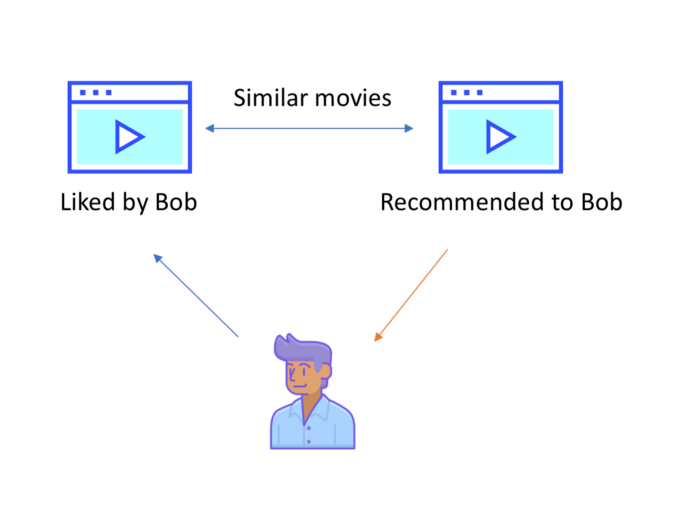
\includegraphics[width=0.5\textwidth]{images/Content-based filtering.png}
            \end{center}
      \end{figure}\\
      The \underline{advantages} of this approach are:
      \begin{itemize}
            \item User autonomy:The model doesn't need any data about other users, since the recommendations are specific to this user. This makes it easier to scale to a large number of users.\\The model can capture the specific interests of a user, and can recommend niche items that very few other users are interested in.
            \item Immediate consideration of a new item: The model does not need the evaluation of all movie by a user, because it can be recommended without being evaluated.
      \end{itemize}
      The \underline{limitations} of this approach are:
      \begin{itemize}
            \item Content too specific: The model can only make recommendations based on existing interests of the user. In other words, the model has limited ability to expand on the users' existing interests.
            \item Big scale information: Since the feature representation of the items are hand-engineered to some extent, this technique requires a lot of domain knowledge. The items must be enouth detailed descripted and a user must evaluate several items before the system can iterpret its preferences.
      \end{itemize}
\end{itemize}
It is also possible to combine these two class of recommendation in order to overcome some limitations they faced. This type of approach is called \textbf{Hybrid Recommendation}.\\
In this project the items that has been evaluated are movies, and their scores are the rating that the users gave after they whatched them.

\newpage

%------------------------------------------%
\section{Objectives}

The purpose of this project is to develop a recommender system, which predicts the ratings of a user towards a domain-specific item. In our case, this domain-specific item is a movie, and the main focus of our recommendation system is to filter and predict only those movies that a user would prefer. The approach chosen to develop this system is a hybrid one. At first, we used a collaborative filtering technique to make predictions on movies' ratings deducted from similarities between users. Then we adopted a content-based filtering technique to predict some movies' ratings based on similarities between movies. The based knowledge of our system derives a data set that is described thoroughly in the next section, while in the fourth section there is a step-by-step description of the algorithm, followed by an evaluation of its performance and an example of output it generates.

%------------------------------------------%
\section{Dataset description}
The data provided are stored in two CSV files named movies.csv and ratings.csv.

\subsection{Movies}
In this dataset are stored information about the movies. The content is structured in 3 different columns : \\
the \textbf{id}, the \textbf{title}, and a list of \textbf{genres}; each row represents a movie. In it are stored 10329 movies with 20 different genres:\\ Western, Documentary, Children, Crime, Film-Noir, Comedy, Adventure, Fantasy, Horror, Thriller, Mystery, Sci-Fi, Musical, Romance, Action, Animation, IMAX, Drama, War, not-defined. \\
In the following image there is a representation of it:
\begin{figure}[ht]
      \begin{center}
            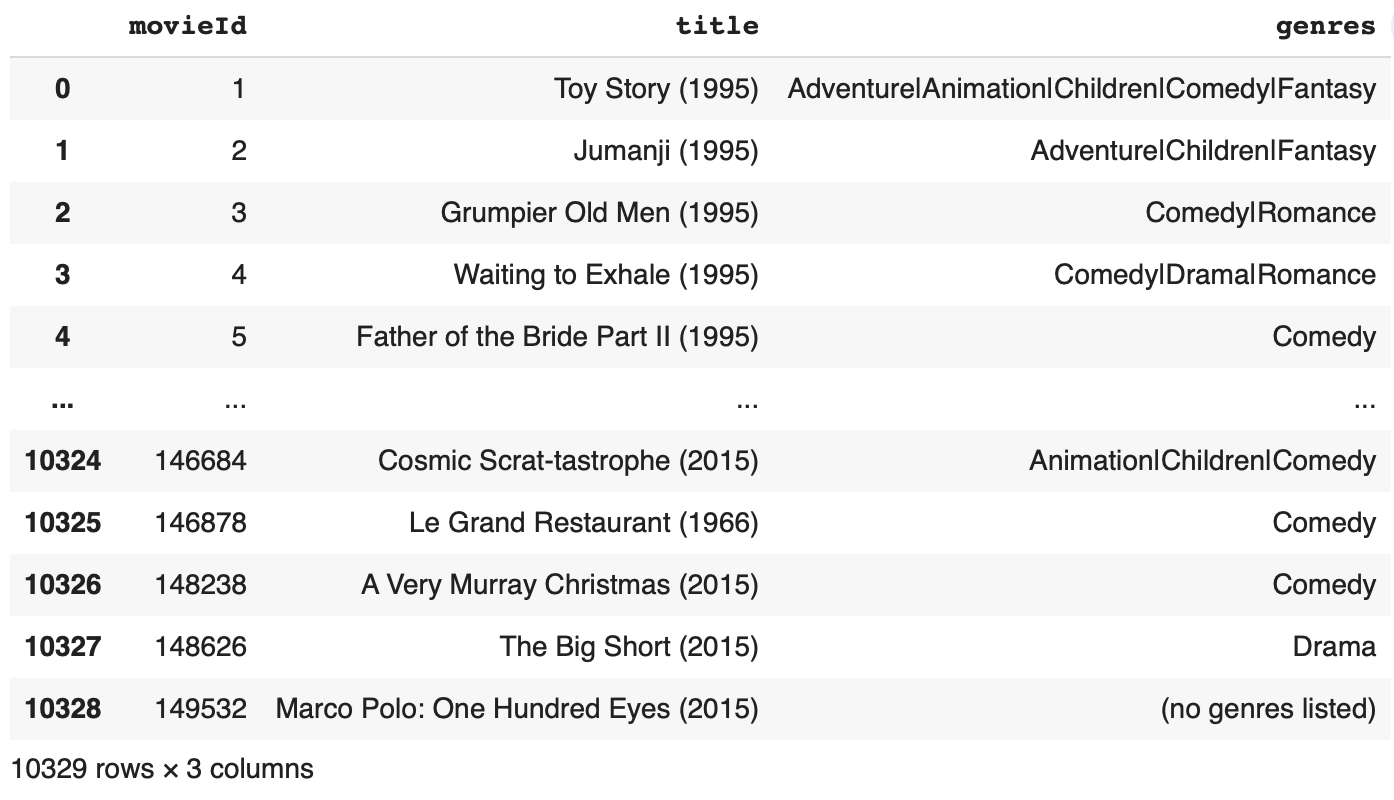
\includegraphics[width=0.5\textwidth]{images/movies data.png}
      \end{center}
\end{figure}

\subsection{Ratings}
Here are stored all the ratings that the users gave to the movies from 0.5 to 5. The 4 columns are filled with respectively: \\the id of a \textbf{user}, the id of a \textbf{movie}, the value of the \textbf{rate} given by the user on the movie and the \textbf{timestamp} (day and time) of the evaluation. Counting the different userId, there are 668 users that overall made 105339 ratings. \\
To follow a representation of it:
\begin{figure}[ht]
      \begin{center}
            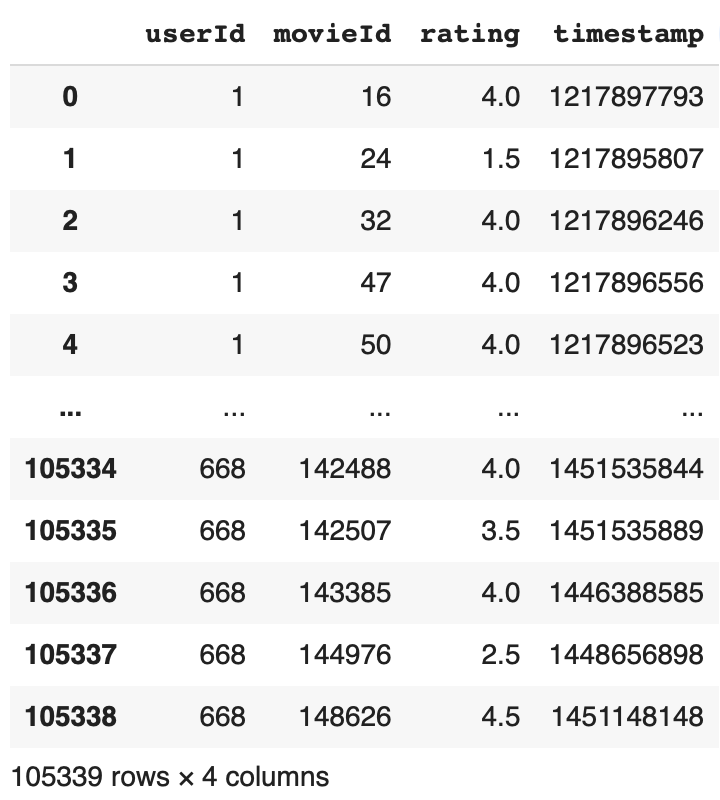
\includegraphics[width=0.4\textwidth]{images/ratings data.png}
      \end{center}
\end{figure}\\
It's also reported the plot of the distribution of the rating data:
\begin{figure}[ht]
      \begin{center}
            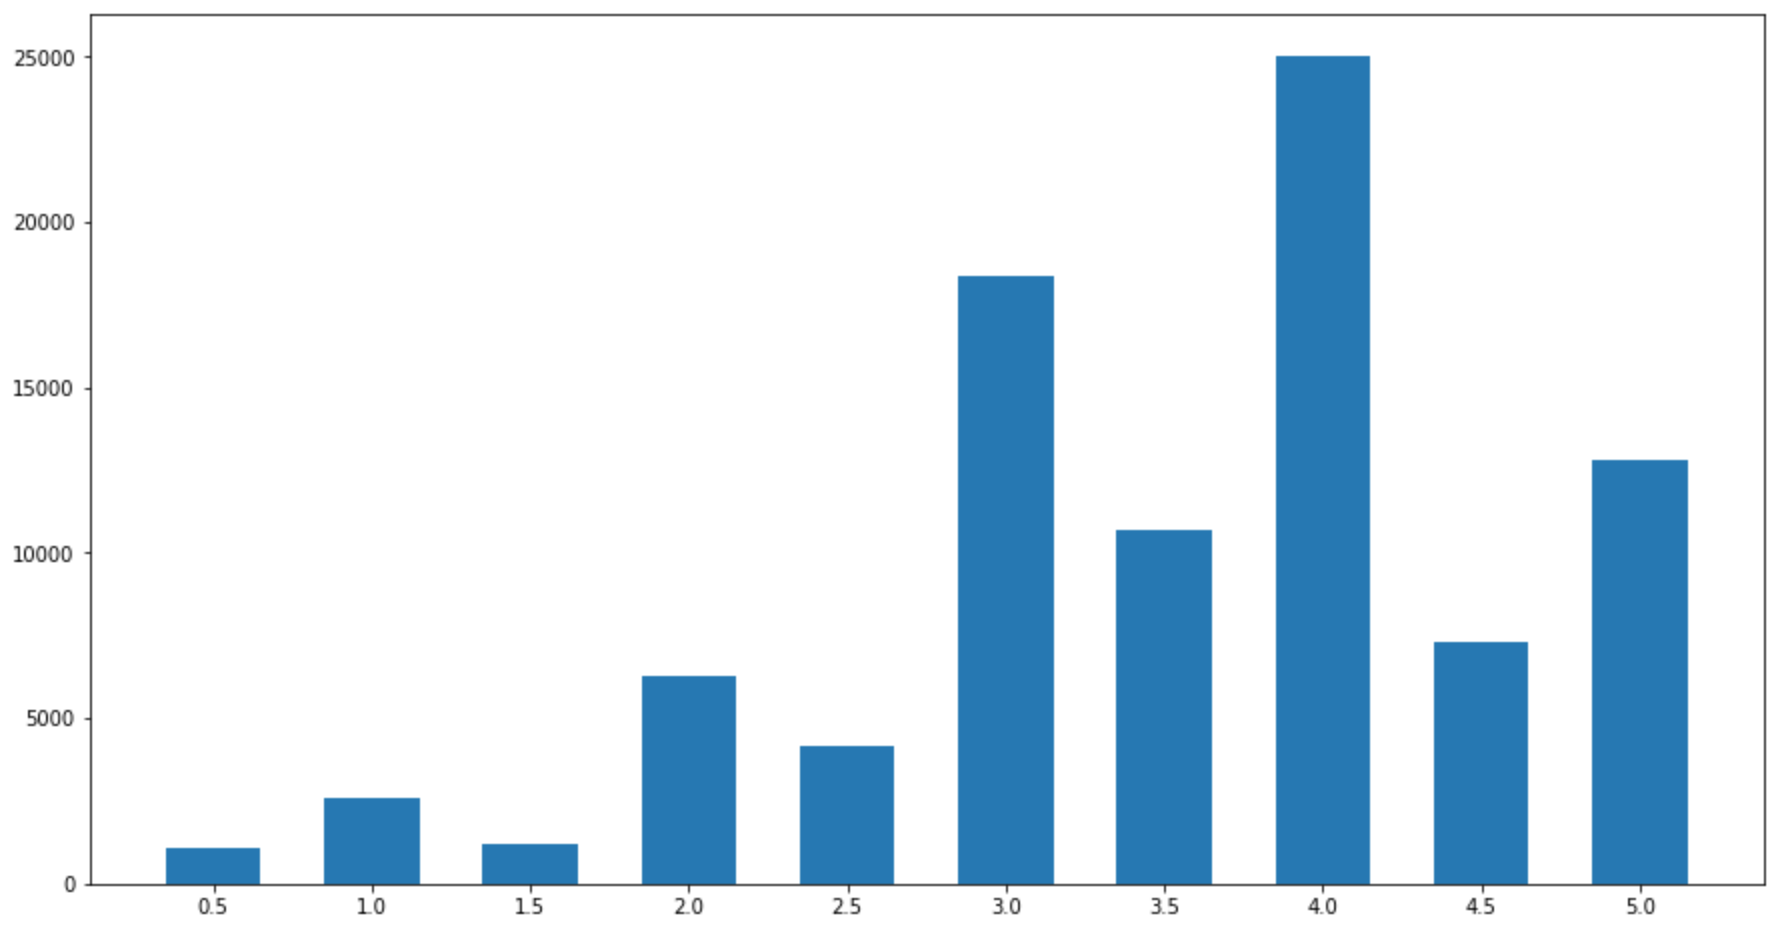
\includegraphics[width=0.8\textwidth]{images/rating distributions.png}
      \end{center}
\end{figure}

\newpage

%------------------------------------------%
\section{Algorithm description}
In this section a detailed step-by-step description of the algorithm adopted is provided.\\
At first, the data has been loaded using the \textsl{pandas} library and then they have been organized in matrices.\\
Before building the matrices, the data has been split:
\begin{itemize}
      \item 80\% as training set
      \item 20\% as testing set
\end{itemize}
It is necessary to shuffle the data before, or in the test set would be only the data about lasts users; the analysis would not be correct.\\ \\
The first matrix called \textbf{ratings matrix} have all the 668 \textbf{user ids} as rows, 10329 \textbf{movie ids} as columns and as values the \textbf{ratings} that users gave to the movies (the ones missing are set to 0.0).\\
\begin{center}
      \begin{tabular}{ | c | c | c | c | c | c | c |} 
        \hline
        \rowcolor{lightgray}  & 1 & 2 & 3 & ... & 148626 & 149532 \\ 
        \hline
         \cellcolor{lightgray}1 & 0.0 & 0.0 & 0.0 &  & 0.0 & 0.0 \\ 
        \hline
        \cellcolor{lightgray}2 & 0.0 & 0.0 & 2.0 &  & 0.0 & 0.0 \\ 
        \hline
        \cellcolor{lightgray}3 & 0.0 & 0.0 & 0.0 &  & 0.0 & 0.0\\
        \hline
        \cellcolor{lightgray}4 & 0.0 & 0.0 & 0.0 &  & 0.0 & 0.0\\
        \hline
        \cellcolor{lightgray}... &  &  &  &  &  & \\ 
        \hline
        \cellcolor{lightgray}668 & 0.0 & 3.0 & 0.0 &  & 4.5 & 0.0\\
        \hline
      \end{tabular}
\end{center}

The second matrix keeps track of all the genres associated with a movie: it has \textbf{movie ids} as rows, \textbf{genres} as columns, and as \textbf{values} "1" if the movie is associated to a genre, 0 otherwise. \\

\begin{equation}
      \label{eqn:movieMatrix}
      CorrelationMatrix_{i,j} = \left \{
            \begin{aligned}
                  &1 && \text{if movie i is of genre j}\\
                  &0 && \text{otherwise}
            \end{aligned} \right.
\end{equation} \\ 

\begin{center}
      \begin{tabular}{ | c | c | c | c | c | c | c |} 
        \hline
        \rowcolor{lightgray}  & Comedy & Drama & Horror & ... & Fantasy & Sci-Fi \\ 
        \hline
         \cellcolor{lightgray}1 & 1 & 0 & 0 &  & 1 & 0 \\ 
        \hline
        \cellcolor{lightgray}2 & 0 & 0 & 0 &  & 1 & 0 \\ 
        \hline
        \cellcolor{lightgray}3 & 1 & 0 & 0 &  & 0 & 0\\
        \hline
        \cellcolor{lightgray}4 & 1 & 1 & 0 &  & 0 & 0\\
        \hline
        \cellcolor{lightgray}... &  &  &  &  &  & \\ 
        \hline
        \cellcolor{lightgray}149532 & 0 & 0 & 0 &  & 0 & 0\\
        \hline
      \end{tabular}
\end{center}

\newpage
\subsection{Binary search}
Binary search is an algorithm that find an element in an array with a complexity of O(log n). It searches in a sorted array by repeatedly dividing the search interval in half. Begin with an interval covering the whole array. If the value of the search key is less than the item in the middle of the interval, narrow the interval to the lower half. Otherwise, narrow it to the upper half. Repeatedly check until the value is found or the interval is empty.
This algorithm is been used to speed up the creation of the training lists with values the indexes they refer to.\\

\subsection{Cosine similarity}
It gives a measure of similarity between two non-zero vectors of an inner product space.\\It calculate the cosine of the angle($\theta$) between them, which is also the same as the inner product of the same vectors normalized to both have lenght 1. \\
\begin{figure}[ht]
      \begin{center}
            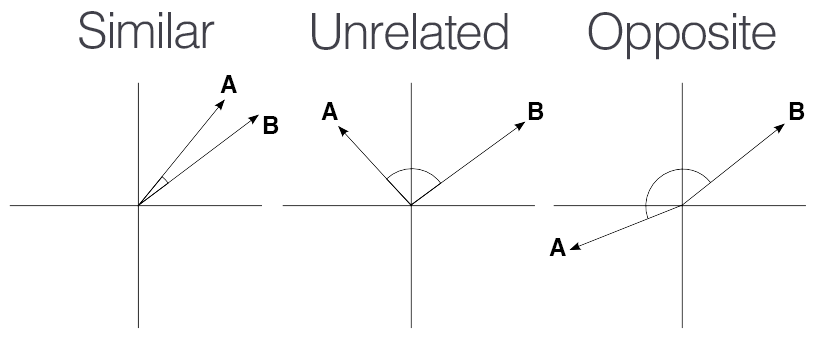
\includegraphics[width=0.6\textwidth]{images/cosine.png}
      \end{center}
\end{figure}\\
Because of that it is bounded in the interval [-1,1] for any angle $\theta$ :
\begin{itemize}
      \item two vectors with the same orientation have a cosine similarity of \textbf{1}
      \item two vectors oriented at right angle relative to each other have a similarity of \textbf{0}
      \item two vectors diametrically opposed have a similarity of \textbf{-1}
\end{itemize}
By using the Euclidean dot product formula:\\
A $\cdot$ B = $\|A\|$ $\|B\|$ $\cos\theta$ \\
We obtain the cosine similarity formula:\\
\begin{equation}
      S_c(A,B) = \cos\theta = \frac{A \cdot B}{\|A\| \|B\|} = \frac{\sum_{i=1}^n A_i B_i}{\sqrt{\sum_{i=1}^n A_i^2}\sqrt{\sum_{i=1}^n B_i^2}}
\end{equation}\\
where $A_i$ anf $B_i$ are components of vector A and B respectively.\\ \\


\subsection{User-User \& Movie-Movie similarity}
For the evaluation of the similarities between movies it's been used the cosine similarity formula between rows of the \textbf{correlation matrix}. For the evaluation of the users similarities the formula is been applied using rows of the \textbf{ratings matrix} but considering only movies rated by both the users (in order to be considered similar they must have at least five common ratings).\\

\subsection{Clustering}
In order to maintain all the similarity between users and movies to avoid later calculation, user's clusters and movie's clusters were created.\\
Algorithm used for the building of the user's clusters(analogous for the movie):
\begin{itemize}
    \item Create a list of user id
    \item Take the first element of the list and check which one of the others in the list is similar
    \item Add all the similar found in a new cluster and delete them from the list
    \item Repeat until the list is empty
\end{itemize}

\newline
In particular, to store the clusters, 2 dictionaries have been used: one containing all the user's clusters and one containing all the movie's clusters. Their structure is the same, the key is the number of the cluster and the value is a list containing the ids of all the elements belonging to the cluster. Furthermore, other two dictionaries have been created for maintaining a direct access to clusters given the id of an element(user or movie): the key is the id and the value is the number of its cluster. 
\newline
This technique it's cheaper from the computation and from the memory point of view and it allows to reduce the workload of the future operations since all the similarities have already been calculated and stored.


\subsection{Collaborative filtering}
Fill the \textbf{ratings matrix}, predicting some missing values given similar behaviour between users:
\begin{itemize}
    \item Given a user, take all the similar in his cluster
    \item First variant: for each movie, calculate the mean rating between all the ratings given by similar users and assign it to the user.\\
    Second variant: for each movie, calculate the mean rating between the most common ratings given by similar users and assign it to the user
    \item Repeat for each user
\end{itemize}


\subsection{Content-based filtering}
Given the matrix filled with some values due to the collaborative filtering, try to predict other ratings with a content-based filtering technique between movies:
\begin{itemize}
    \item Take a user (a row of the \textbf{ratings matrix}) and retrieve all the movies' clusters
    \item For each cluster
    \subitem Calculate the average rating given by the user (ratings $\ge$ 0.5) only to movies that belongs to the cluster;
    \subitem Insert the average in the position corresponding to movies of the current cluster not rated yet by the user or, if it's not rated but predicted by the collaborative filtering, insert the mean between them
\end{itemize}


\subsection{SVD}
In linear algebra, the singular value decomposition (SVD) is a factorization of a real or complex matrix. It generalizes the eigendecomposition of a square normal matrix with an orthonormal eigenbasis to any m × n matrix.
\begin{equation}
      S = U\Sigma V^T
\end{equation}
Specifically, the singular value decomposition of an m $\times$ n complex matrix S is a factorization of the form U$\Sigma V^T$, where \textbf{U} is an m $\times$ m complex unitary matrix, \textbf{$\Sigma$} m $\times$ n rectangular diagonal matrix with non-negative real numbers on the diagonal, and \textbf{V} is an n $\times$ n complex unitary matrix.\\
The diagonal entries $\sigma _{i}$ = $\Sigma _{ii}$ of $\Sigma$ are known as the singular values of S. The number of non-zero singular values is equal to the rank of S. The columns of U and the columns of V are called the left-singular vectors and right-singular vectors of S, respectively.\\

\subsubsection{SVT}
The singular value truncation (SVT) uses the idea of SVD to complete the original matrix. In particular, it's a recursive process that calculate the SVD of the matrix and then try to reduce its rank modifying the singular values in $\Sigma$.Finally reconstruct the matrix using the same \textbf{U} and \textbf{V} but with the new $\Sigma$. In the algorithm used the singular values are modified according to an adaptive threshold: it's value depends on the number of iteration done. A constant threshold is also possible, for example threshold = 50 gave good results\newline

Here are reported the main steps of the algorithm used:

\begin{itemize}
    \item Copy the current matrix (the \textbf{old matrix})
    \item Perform the SVD: \begin{equation}X = U\Sigma V^T\end{equation}
    \item Calculate the threshold for this step: \begin{equation}
        threshold = b * e^{(-k * a)}
    \end{equation}\\
    where k is the number of iterations already done, a = 0.01, b = 200
    \item To each singular values greater than zero subtract the threshold and set to zero the ones that become negative
    \item Build the \textnbf{new matrix} performing the SVD using the same U and V obtained by the initial decomposition and the diagonal matrix $\Sigma$ with the new singular values
    \item Update the new matrix obtained in the previous point with the values fixed before the application of the algorithm: the true ratings and the ones predicted
    \item If there are negative values in the new matrix, set them to zero
    \item Calculate the increment: the difference in module between the \textnbf{new matrix} and the \textnbf{old matrix}
    \item Repeat until k is lesser than the maximum number if iterations available and the increment is greater than epsilon, where their values are, respectively, 100 and 0.1
\end{itemize}

\subsection{Neural Network}
Instead of using collaborative and content-based filtering, it's also possible to use Neural Networks to do it implicitly. In the second solution provided it's been created a neural network for each user. Each NN is been trained using SGD with momentum using two differnte type of data:

\begin{itemize}
    \item Input: a vector for each movie directly rated by the user (the vector correspond to a row of the \textnbf{correlation matrix}).\newline
    Output: a vector of 10 position for each movie, where each position corresponds to a rating (from 0.5 to 5) and with all zero except in the position corresponding to the right rate where there is 1
    \item The same but with movies the uses hasn't rated. In this case, ratings of similar users are been used
\end{itemize}

\subsubsection{Structure of the neural network}

\subsubsection{Activation function}

\subsubsection{Optimization method}

\subsubsection{Loss function}

\subsection{Possible improvements}
Maybe say it in the end! To complete!
In order to improve the performance is also possible to use the timestamp of each rating to find better similarities to users, for example to give more importance to users who rated the same movie more or less in the same days/months with respect to users who rated the same movies with many years between them



\newpage

%------------------------------------------%
\section{Results}
From the result obtained get an example: from one user, his ratings, the first 10 movie our system would reccommend

\subsection{Error calculation}
Compare the results obtained with the dataset part kept apart for the testing

\subsubsection{RMSE}

Root Mean Square Error (RMSE) is the standard deviation of the residuals (prediction errors). Residuals are a measure of how far from the regression line data points are; RMSE is a measure of how spread out these residuals are. In other words, it tells you how concentrated the data is around the line of best fit. 

The formula is:
\begin{equation}
      RMSE = \sqrt{\frac{1}{|\Omega_{test}|}\sum_{i,j\in\Omega_test} (r_{i,j} - r_{i,j}^{pred})}
\end{equation}
\subsubsection{rho}
Pearson correlation coefficient is a measure of linear correlation between two sets of data. It is the ratio between the covariance of two variables and the product of their standard deviations; thus it is essentially a normalised measurement of the covariance, such that the result always has a value between −1 and 1. As with covariance itself, the measure can only reflect a linear correlation of variables, and ignores many other types of relationship or correlation.
It is calculated as follow:
\begin{equation}
      \rho = \frac{\sum_{\Omega_{test}} (r_{ij}-\overline{r})(r_{ij}^{pred}-\overline{r^{pred}})}{{\sqrt{\sum_{\Omega_{test}}(r_{ij}-\overline{r})^2}}{\sqrt{\sum_{\Omega_{test}}(r_{ij}^{pred}-\overline{r^{pred}})^2}}}
\end{equation}
The result is a value between [-1,1]:
\begin{itemize}
      \item 1 = perfect match-strong positive relation; all data points lie on a line for which both variable r and $r_{pred}$ are increasing
      \item 0 = random; there is no linear dependency between the variables
      \item -1 = strong negative relation; also here a linear equation describes the relationship between the variables r and $r_{pred}$ and the points lie on a line in which are decreasing
\end{itemize}
\begin{figure}[ht]
      \begin{center}
            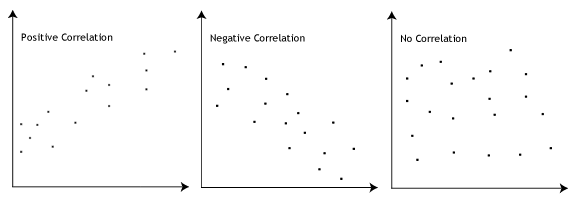
\includegraphics[width=0.6\textwidth]{images/pearson.png}
      \end{center}
\end{figure}

\subsection{Precision}
Precision tries to answer the following question:\\
'What proportion of positive identification was actually correct?'

\begin{equation}
      Precision = \frac{TP}{TP + FP}
\end{equation}
\subsection{Recall}
Recall tries to answer the following question:\\
'What proportion of actual positives was identified correctly?'

\begin{equation}
      Recall = \frac{TP}{TP + FN}
\end{equation}

\subsection{F1-measure}
It's a measure given by the relation between precision and recall
\begin{equation}
    F1-score = 2 \times \frac{Precision x Recall}{Precision + Recall}
\end{equation}
\end{document}